% Settings for the default beamer theme
\documentclass[english, aspectratio=169]{beamer}
\usepackage[T1]{fontenc}
\usepackage[utf8]{inputenc}
\usepackage{adjustbox}
\usepackage{tabularx}
\usepackage{listings}
\usepackage{graphicx}
\usepackage{array}
\usepackage{babel}
\usepackage[ruled,vlined]{algorithm2e}
\usepackage{blkarray}
\SetAlgorithmName{Algoritmus}{algoritmus}{List of Algorithms}
\setcounter{secnumdepth}{3}
\setcounter{tocdepth}{3}


\makeatletter

\newcommand\makebeamertitle{\frame{\maketitle}}

% (ERT) argument for the TOC
\AtBeginDocument{%
  \let\origtableofcontents=\tableofcontents
  \def\tableofcontents{\@ifnextchar[{\origtableofcontents}{\gobbletableofcontents}}
  \def\gobbletableofcontents#1{\origtableofcontents}
}

% Theme settings
\usetheme{Frankfurt}
\usecolortheme{default}
\usefonttheme[onlymath]{serif}

% Template settings
\setbeamertemplate{navigation symbols}{}
\setbeamertemplate{blocks}[rounded][shadow=false]
\setbeamertemplate{title page}[default][colsep=-4bp, rounded=true, shadow=false]
\makeatother

% Custom color definitions
\definecolor{lightgrey}{gray}{0.95}
\definecolor{DarkerGreen}{RGB}{0,85,0} % Adjust the RGB values as needed

% Use the newly defined color in Beamer theme elements
\setbeamercolor{structure}{fg=DarkerGreen} % Changes basic structural elements to Darker Green
\setbeamercolor{title in head/foot}{bg=DarkerGreen} % Changes the title in header/footer to Darker Green

% Definitions for program code sections
\lstset{
	language=bash,
	basicstyle=\ttfamily\footnotesize, % Monospace font
	backgroundcolor=\color{lightgrey}, % Background color
	frame=single, % Frame around the code
	keywordstyle=\color{black}, % Keywords color
	commentstyle=\color{black}, % Comments color
	stringstyle=\color{red}, % Strings color
	showstringspaces=false, % Do not show spaces in strings
	breaklines=true, % Automatically break long lines
}

\lstset{
	language=python,
	basicstyle=\ttfamily\scriptsize, % Basic font style
	keywordstyle=\bfseries\color{blue}, % Keywords in bold and blue
	stringstyle=\color{red}, % Strings in red
	commentstyle=\color{green!50!black}, % Comments in green
	showstringspaces=false, % Do not show spaces in strings
	numbers=left, % Line numbers on the left
	numberstyle=\tiny\color{gray}, % Line number style
	stepnumber=1, % Line number step
	numbersep=5pt, % Distance of line numbers from code
	frame=single, % Frame around the code
	rulecolor=\color{black}, % Frame color
	tabsize=2, % Tab size
	breaklines=true, % Automatic line breaking
	breakatwhitespace=false, % Break lines at whitespace
	captionpos=b, % Caption position
	escapeinside={\%*}{*)}, % Escape to LaTeX
	morekeywords={self}, % Additional keywords
	literate={á}{{\'a}}1
	{é}{{\'e}}1
	{í}{{\'i}}1
	{ó}{{\'o}}1
	{ú}{{\'u}}1
	{ő}{{\H{o}}}1
	{ű}{{\H{u}}}1
	{Á}{{\'A}}1
	{É}{{\'E}}1
	{Í}{{\'I}}1	
	{Ó}{{\'O}}1	
	{Ú}{{\'U}}1
	{Ő}{{\H{O}}}1
	{Ű}{{\H{U}}}1
	{Ö}{{\"O}}1
	{Ü}{{\"U}}1
	{ö}{{\"o}}1
	{ü}{{\"u}}1
}


\begin{document}

% Title page
\section{Dinamikus felhasználói komponensek}
\title[]{Adatbányászat a Gyakorlatban}
\subtitle{6. Gyakorlat: Haladó Dash módszerek}
\author[Kuknyó Dániel]{Kuknyó Dániel\\Budapesti Gazdasági Egyetem}
\date{2024/25\\1.félév}
\makebeamertitle

% Table of contents slide
\begin{frame}
\tableofcontents{}
\end{frame}

% Table of contents of the current section
\begin{frame}
\tableofcontents[currentsection]
\end{frame}

\begin{frame}[fragile]{Dinamikus felhasználói komponensek (\texttt{dyn\_component\_app\_v1.py})}
	\begin{columns}
		\begin{column}{.5\textwidth}
			Olyan dinamikus komponensek, amelyek nem állandóak, hanem felhasználói interakcióra kerülnek hozzáadásra az alkalmazáshoz, és el is lehet őket távolítani.\par\smallskip
			Ehhez tartozóan az első alkalmazás elrendezése:\par\smallskip
			\begin{lstlisting}[language=python]
app.layout = html.Div([
	dbc.Button("Diagram hozzáadása", id='dyn_component_button'),
	html.Div(id='dyn_component_output', children=[]),
])
			\end{lstlisting}
		\end{column}
		\begin{column}{.5\textwidth}
			\begin{center}
				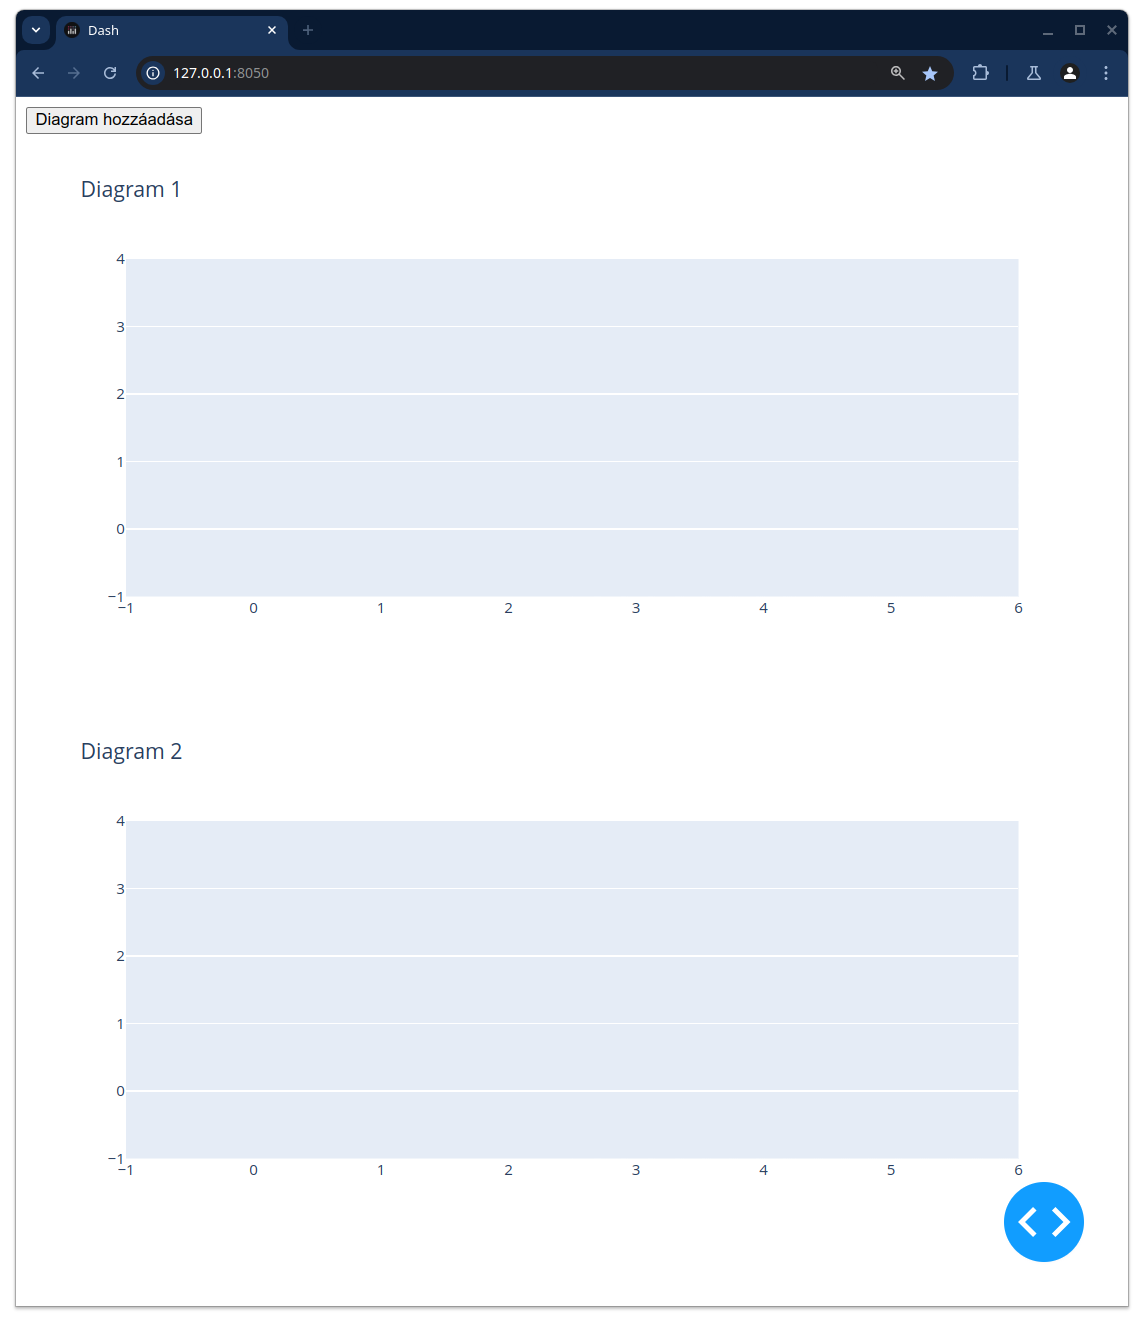
\includegraphics[width=7cm, height=7cm, keepaspectratio]{images/adv_1.png}
			\end{center}
		\end{column}
	\end{columns}
\end{frame}

\begin{frame}[fragile]{Callback függvény felhasználói komponensek hozzáadására}
	\begin{columns}
		\begin{column}{.5\textwidth}
			A callback a \texttt{dyn\_component\_output} \texttt{Div} \texttt{children} komponensét frissíti.\par\medskip
			Ha a gombot megnyomták, létrehoz egy új oszlopdiagramot, és a diagram címében megjeleníti a gombnyomások számát.
			Az új diagramot hozzáadja a \texttt{children} listához.\par\medskip
			Visszatér a frissített \texttt{children} listával, amely tartalmazza az új diagramot.
		\end{column}
		\begin{column}{.5\textwidth}
			\begin{lstlisting}[language=python]
@app.callback(
	Output('dyn_component_output', 'children'),
	Input('dyn_component_button', 'n_clicks'),
	State('dyn_component_output', 'children')
)
def add_new_chart(n_clicks, children):
	if not n_clicks:
		return no_update
	new_chart = dcc.Graph(figure=px.bar(title=f"Diagram {n_clicks}"))
	children.append(new_chart)
	return children

			\end{lstlisting}
		\end{column}
	\end{columns}
\end{frame}

\begin{frame}{Az alkalmazás callback gráfja}
	A callback gráf ebben az esetben egy speciális hurkot mutat. Ez azt jelenti, hogy a függvény egy olyan komponenst térít vissza, amit megkapott paraméterül és módosított a függvénytörzsben.\par\smallskip
	Ez a diagram változatlan marad a hozzáadott komponensek számától függetlenül.
	\vspace{1cm}
	\begin{center}
		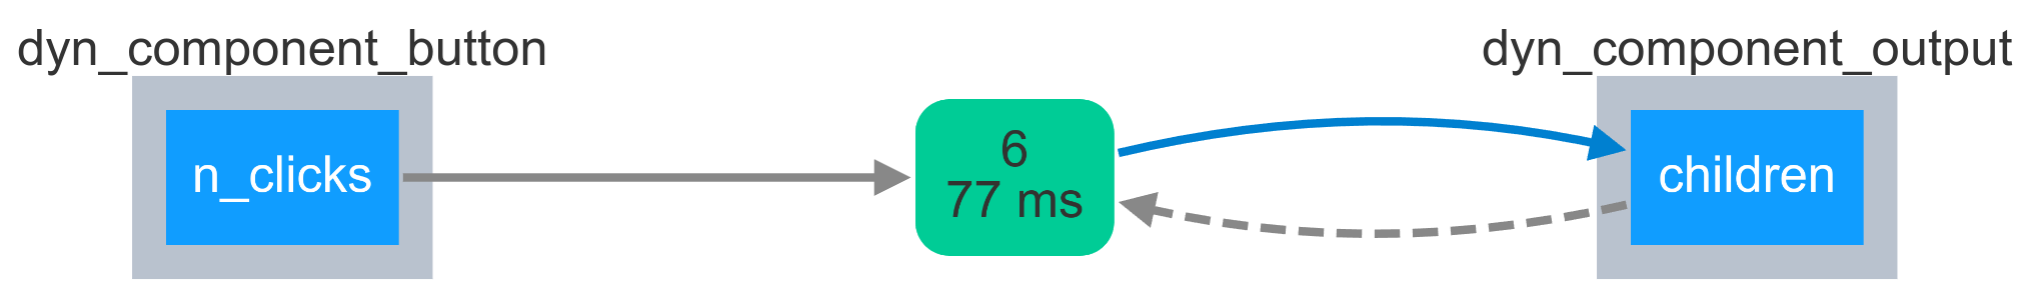
\includegraphics[width=10cm, height=7cm, keepaspectratio]{images/adv_2.png}
	\end{center}
\end{frame}

\begin{frame}[fragile]{Mintaillesztő callback függvények}
	\begin{columns}
		\begin{column}{.5\textwidth}
			Az alkalmazás következő verziója interaktivitást ad a felhasználói komponenseknek, mintaillesztő callback függvények segítségével.\par\smallskip
			Minden diagramnak van egy saját legördülő menüje, ahol ki lehet választani egy országnevet, majd kirajzolja a népességet a diagramra. 
		\end{column}
		\begin{column}{.5\textwidth}
			\begin{center}
				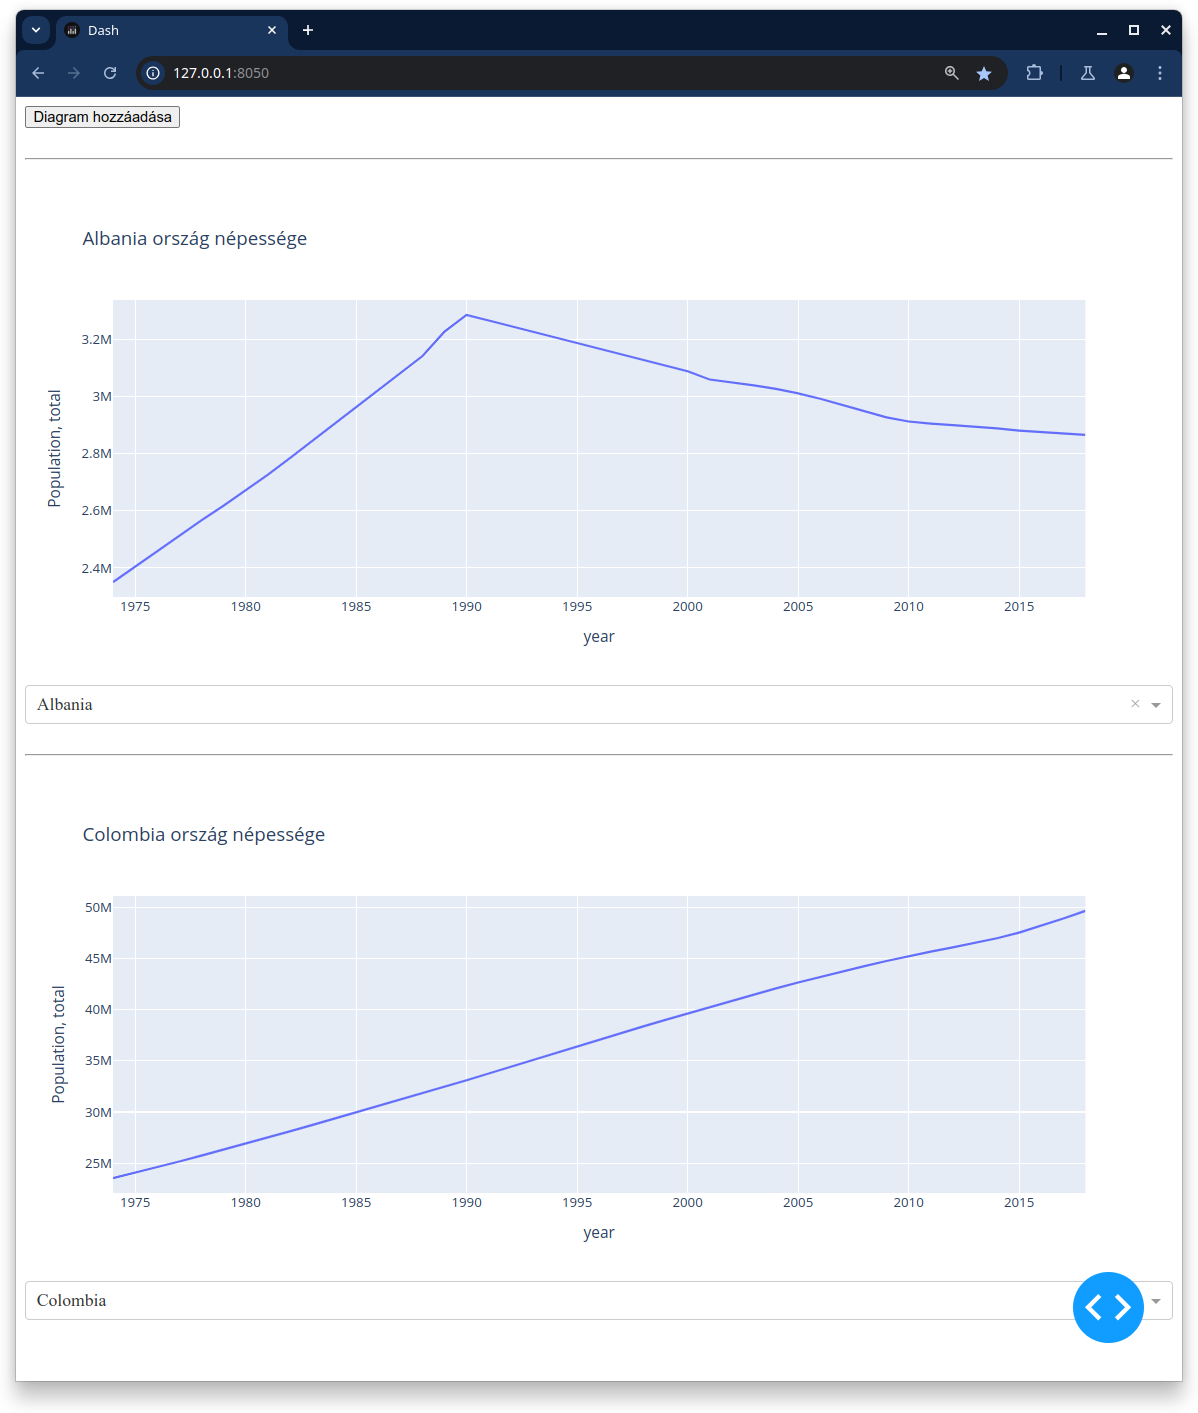
\includegraphics[width=7cm, height=7cm, keepaspectratio]{images/adv_3.png}
			\end{center}
		\end{column}
	\end{columns}
\end{frame}

\begin{frame}[fragile]{Dinamikus komponens elnevezések}
	\begin{columns}
		\begin{column}{.5\textwidth}
			Dash rendszerben egy komponens \texttt{id} paramétere bármilyen hash-képes (egy függvényen keresztül egyértelműen leképezhető) objektum lehet, így pl. egy szótár is.\par\smallskip
			Az alkalmazásban a \texttt{id} attribútum egy szótár, amely tartalmazza a \texttt{type} és \texttt{index} kulcsokat. Ez a struktúra lehetővé teszi komponenseket dinamikus azonosítását az alkalmazásban. Például több diagram létrehozása és módosítása esetén mindegyiket egyedi névvel látja el.  
		\end{column}
		\begin{column}{.5\textwidth}
			\begin{lstlisting}[language=python]
# Új diagram létrehozása
new_chart = dcc.Graph(
	id={'type': 'chart', 'index': n_clicks},
	figure=px.bar(title=f"Diagram {n_clicks}")
)
# Legördülő lista opciók létrehozása
countries = poverty[poverty['is_country']]['Country Name'].drop_duplicates().sort_values()
# Legördülő lista létrehozása
new_dropdown = dcc.Dropdown(
	id={'type': 'dropdown', 'index': n_clicks},
	options=[{'label': c, 'value': c} for c in countries],
	placeholder='Ország kiválasztása'
)
			\end{lstlisting}
		\end{column}
	\end{columns}
\end{frame}

\begin{frame}[fragile]{Dash \texttt{MATCH}}
	\begin{columns}
		\begin{column}{.5\textwidth}
			A \texttt{dash.dependencies.MATCH} lehetővé teszi, hoyg a callback egy adott komponenscsoport egy adott példányára vonatkozzon.\par\medskip
			Például ha több dinamikus objektum közül mindegyiknek van egy egyedi \texttt{id} paramétere egy szótár formájában, akkor a \texttt{MATCH} segítségével meg lehet határozni, hogy a callback csak az adott indexnek megfelelő komponensre reagáljon.
		\end{column}
		\begin{column}{.5\textwidth}
			\begin{lstlisting}[language=python]
@app.callback(
	Output({'type': 'chart', 'index': MATCH}, 'figure'),
	Input({'type': 'dropdown', 'index': MATCH}, 'value'),
)
def create_population_chart(country):
	if not country:
		return no_update
	# Adatkészlet szűrése
	df = poverty[poverty['Country Name'] == country]
	# Diagram létrehozása
	fig = px.line(
		df,
		x='year',
		y='Population, total',
		title=f'{country} ország népessége'
	)
	return fig
			\end{lstlisting}
		\end{column}
	\end{columns}
\end{frame}

\end{document}
































